\documentclass[12pt, a4paper]{article}

% ===== 中文支持 =====
\usepackage[UTF8, zihao=-4]{ctex}

% ===== 页边距（GB/T 7713.1） =====
\usepackage[
  top=2.5cm, bottom=2.5cm,
  left=2.8cm, right=2.8cm
]{geometry}

% ===== 字体 =====
\usepackage{fontspec}
\setmainfont{Times New Roman}

% ===== 行距 =====
\usepackage{setspace}
\setstretch{1.5}
\setlength{\parskip}{0pt}

% ===== 插图 =====
\usepackage{graphicx}
\usepackage{float}
\graphicspath{{./}}

% ===== 表格（三线表） =====
\usepackage{booktabs}
\usepackage{array}
\usepackage{multirow}
\usepackage{siunitx}

% ===== 数学公式 =====
\usepackage{amsmath, amssymb}

% ===== 图表编号（分章） =====
\renewcommand{\thefigure}{\arabic{section}-\arabic{figure}}
\renewcommand{\thetable}{\arabic{section}-\arabic{table}}
\renewcommand{\theequation}{\arabic{section}-\arabic{equation}}
\counterwithin{figure}{section}
\counterwithin{table}{section}
\counterwithin{equation}{section}

% ===== 图表标题格式 =====
\usepackage{caption}
\captionsetup{
  font=small,
  labelsep=space,
  justification=centering,
  aboveskip=6pt,
  belowskip=12pt
}
\captionsetup[table]{
  aboveskip=12pt,
  belowskip=6pt,
  position=above
}

% ===== 页眉页脚 =====
\usepackage{fancyhdr}
\setlength{\headheight}{15pt}
\pagestyle{fancy}
\fancyhf{}
\fancyhead[C]{\small 实验报告}
\fancyfoot[C]{\small\thepage}

% ===== 目录超链接 =====
\usepackage[colorlinks=true, linkcolor=black, citecolor=black, urlcolor=blue,
            bookmarks=true, bookmarksnumbered=true]{hyperref}

% ===== 章节标题格式 =====
\usepackage{titlesec}
\titleformat{\section}[block]
  {\centering\heiti\zihao{4}}{\thesection}{1em}{}
\titlespacing*{\section}{0pt}{24pt}{18pt}
\titleformat{\subsection}[hang]
  {\heiti\zihao{-4}}{\thesubsection}{1em}{}
\titlespacing*{\subsection}{0pt}{18pt}{6pt}
\titleformat{\subsubsection}[hang]
  {\heiti\zihao{-4}}{\thesubsubsection}{1em}{}
\titlespacing*{\subsubsection}{0pt}{12pt}{6pt}

\begin{document}

% ===== 封面 =====
\begin{titlepage}
  \centering
  \vspace*{3cm}
  {\heiti\zihao{2} 实验报告} \\[1cm]
  {\heiti\zihao{3} 光栅参数测量实验} \\[2cm]
  \begin{tabular}{rl}
    姓\quad 名： & 叶哲昊 \\[0.5cm]
    学\quad 号： & 24012561 \\[0.5cm]
    班\quad 级： & \underline{\hspace{4cm}} \\[0.5cm]
    实验日期：   & 2026年4月17日 \\
  \end{tabular}
  \vfill
\end{titlepage}

\tableofcontents
\newpage

% ===== 正文开始 =====
\setcounter{page}{1}

\section{实验目的}

\begin{enumerate}
  \item 了解全息光栅的基本原理，理解光栅的衍射机制；
  \item 掌握光栅方程 $d\sin\theta = k\lambda$ 的应用，测量并计算光栅常数 $d$；
  \item 观察并分析衍射光栅条纹的分布特点，理解光栅的分光性能。
\end{enumerate}

\section{实验原理}

\subsection{光栅的基本特性}

光栅是一种常用的光学色散元件，广义上可定义为：凡是能使入射光的振幅或相位，或者两者同时产生周期性空间调制的光学元件。衍射光栅通常由大量等宽、等间距、平行排列的狭缝（或反射面）构成。光栅常数 $d = a + b$，其中 $a$ 为透光（或反光）部分的宽度，$b$ 为不透光（或不反光）部分的宽度。

光栅按不同方式可分为：振幅型和相位型（按调制方式）；透射型和反射型（按工作方式）；平面光栅和凹面光栅（按工作表面的形状）；机刻光栅、复制光栅和全息光栅（按制作方式）等。

\subsection{光栅方程}

当平行光垂直入射到光栅上时，在衍射角 $\theta$ 方向产生亮条纹的条件为：
\begin{equation}
d \sin\theta = k\lambda \quad (k = 0, \pm 1, \pm 2, \dots)
\label{eq:grating}
\end{equation}
式中 $\theta$ 为衍射角，$\lambda$ 为入射光波长，$k$ 为光谱级次，$d$ 为光栅常数。这就是光栅方程。

当入射光不垂直于光栅平面时（入射角为 $i$），光栅方程应修正为：
\begin{equation}
d(\sin\theta - \sin i) = k\lambda
\label{eq:grating-oblique}
\end{equation}
因此，在使用式 (\ref{eq:grating}) 时，必须保证平行光垂直入射。

在 $\theta = 0$ 处，$k = 0$，任何波长都满足极大条件，出现中央亮条纹（零级）。对于 $k$ 的其他数值，符号 ``$\pm$'' 表示两组光谱由中央亮条纹向左右对称分布。

\subsection{多缝衍射强度分布}

衍射场中 $P$ 点处的光强度为：
\begin{equation}
I = I_0 \left(\frac{\sin\alpha}{\alpha}\right)^2 \cdot \left[\frac{\sin(N\delta/2)}{\sin(\delta/2)}\right]^2
\label{eq:intensity}
\end{equation}
其中 $\alpha = \pi a \sin\theta / \lambda$，$\delta = 2\pi d \sin\theta / \lambda$，$I_0 = A_0^2$ 为单缝中央主极大光强。式中第一项为单缝衍射因子，第二项为多光束干涉因子。多缝衍射是衍射和干涉两种效应共同作用的结果。

各级主极大的强度为 $I = N^2 I_0 (\sin\alpha/\alpha)^2$，表明其强度受衍射因子调制，是单缝衍射在各级主极大位置上产生强度的 $N^2$ 倍。缝数 $N$ 越大，主极大亮纹越亮。

\subsection{极大与极小条件}

当 $\sin(N\delta/2) = 0$ 且 $\sin(\delta/2) \neq 0$ 时，即 $d\sin\theta = (m + m'/N)\lambda$（$m = 0, \pm 1, \pm 2, \dots$；$m' = 1, 2, \dots, N-1$）时，干涉因子为零，出现极小值。在两个相邻主极大之间有 $N-1$ 个零值。

主极大的半角宽度为：
\begin{equation}
\Delta\theta = \frac{\lambda}{Nd\cos\theta}
\label{eq:half-width}
\end{equation}
缝数 $N$ 越大，主极大的宽度越小，衍射条纹越窄越锐。

\subsection{缺级现象}

若干涉因子的某级主极大刚好与衍射因子的某级极小值重合，该级主极大就会消失，称为缺级。缺级条件为：
\begin{equation}
\frac{d}{a} = \frac{m}{n} \quad (n = \pm 1, \pm 2, \dots)
\label{eq:missing}
\end{equation}
$m$ 即为所缺的级次。例如当 $d = 2a$ 时，$\pm 2, \pm 4, \dots$ 级将缺级。

\subsection{光栅的分光性能参数}

\subsubsection{分辨本领}

分辨本领 $R$ 的定义为：
\begin{equation}
R = \frac{\lambda}{\Delta\lambda} = kN = k\frac{l}{d}
\label{eq:resolution}
\end{equation}
式中 $l$ 为受光面宽度。光栅在使用面积一定的情况下，刻线数目越多，分辨率越高。

\subsubsection{角色散率}

角色散率 $D$ 定义为：
\begin{equation}
D = \frac{\Delta\theta}{\Delta\lambda} = \frac{k}{d\cos\theta}
\label{eq:dispersion}
\end{equation}
级次越高、光栅常数越小，角色散率越大。

\section{实验仪器}

本实验使用的主要仪器和光学元件包括：
\begin{itemize}
  \item He-Ne激光器（波长 $\lambda = \SI{532}{nm}$）
  \item 衰减片
  \item 空间滤波器（针孔滤波器）
  \item 准直透镜（准直镜）
  \item 可调光阑
  \item 透射光栅（全息光栅）
  \item 聚焦透镜
  \item 白屏（带刻度尺）
  \item 卷尺
  \item 光学平台（防震台）及支架
\end{itemize}

\section{实验步骤}

\subsection{实验一：$\pm$5级光栅常数测量}

在激光器后依次放置衰减片、空间滤波器、准直镜、可调光阑、透射光栅、聚焦透镜和白屏。使扩束准直后的均匀激光束照射在光栅上，调节白屏与聚焦透镜的距离至焦平面位置，分别测量 $\pm 1$、$\pm 2$、$\pm 3$、$\pm 4$、$\pm 5$ 级衍射图像的位置，记录各级亮斑到零级中心的距离。

实验一光路搭建如图 \ref{fig:setup1} 所示。

\begin{figure}[H]
\centering
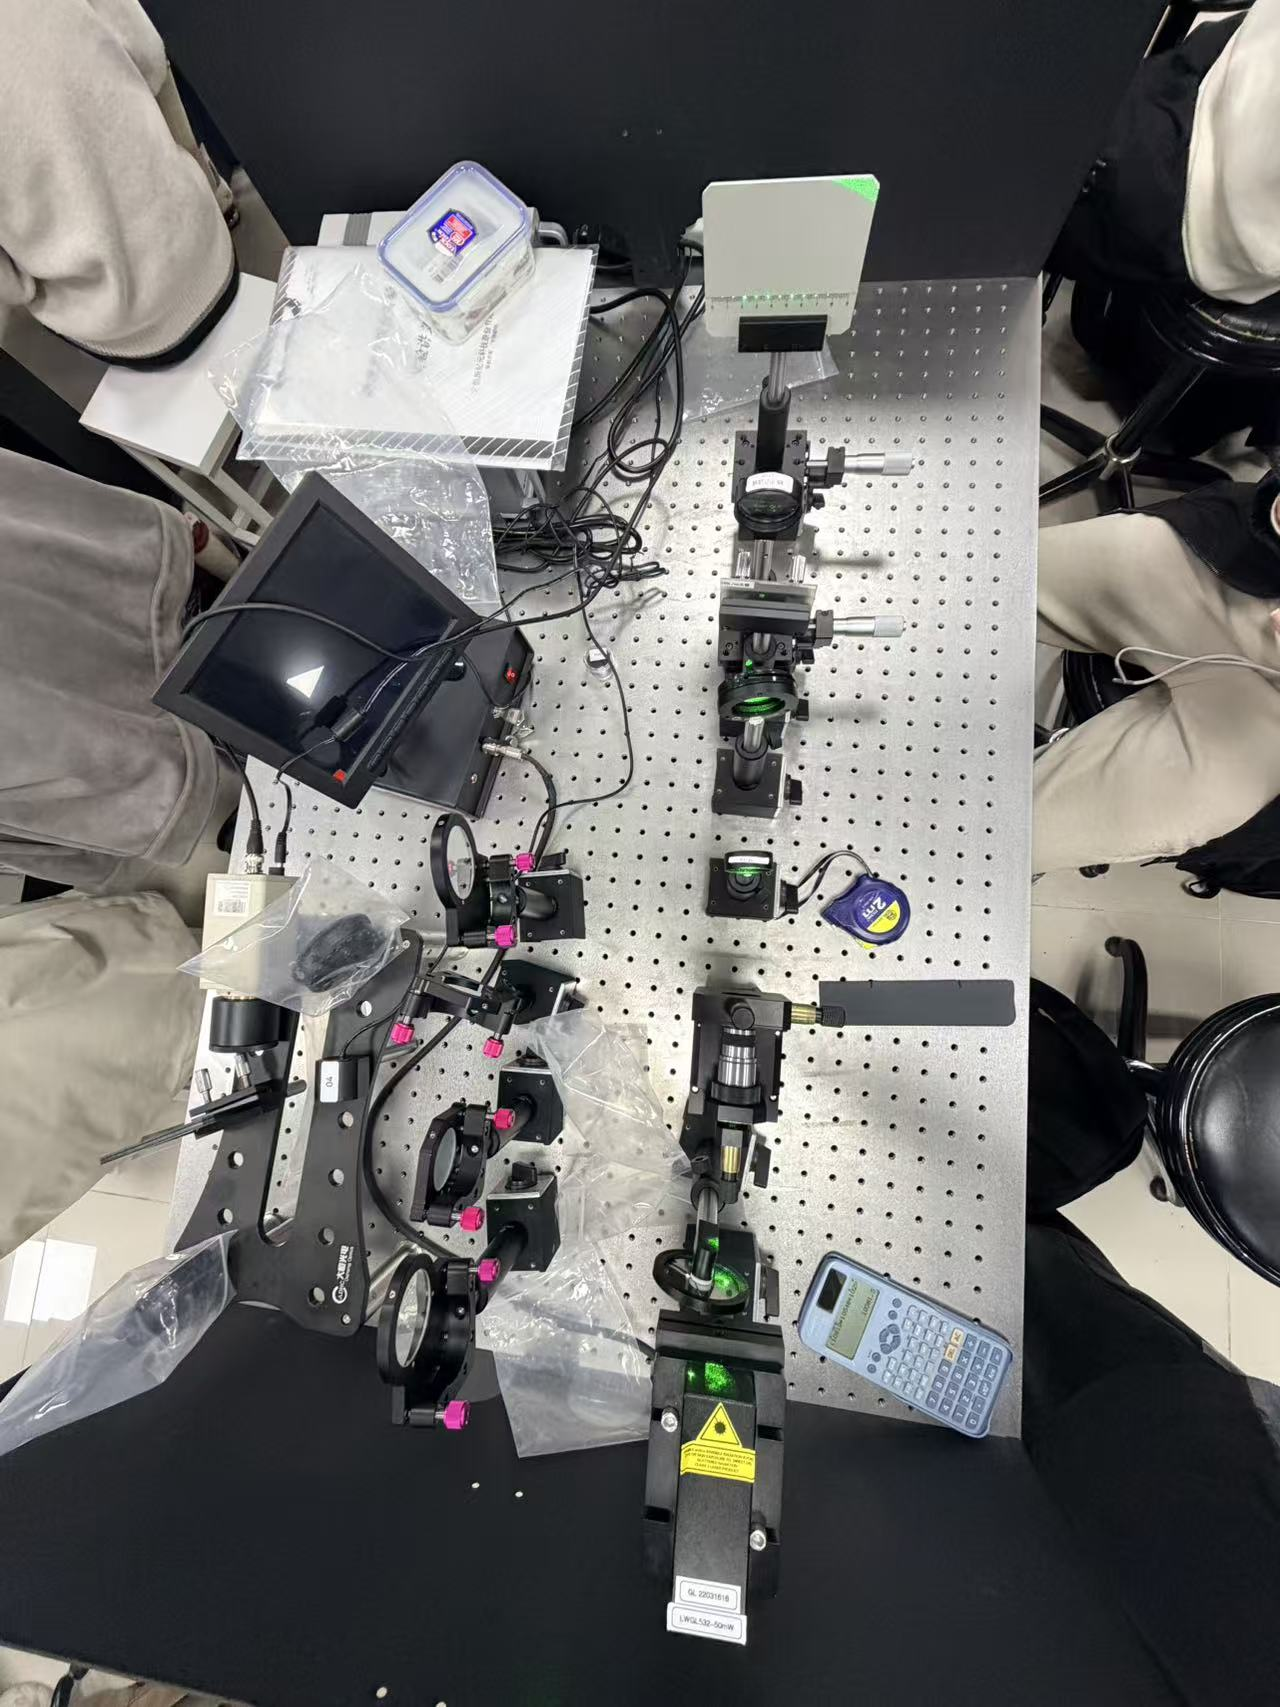
\includegraphics[width=0.75\textwidth]{实验图片/实验一装置完整实物光路搭建.jpg}
\caption{实验一光路实物图}
\label{fig:setup1}
\end{figure}

\subsection{实验二：$\pm$1级光栅常数测量}

在激光器后放置衰减片，使激光束垂直直接照射在光栅上，用卷尺量取光栅到白屏的距离 $L$。通过白屏上的刻度读出 $+1$ 级和 $-1$ 级衍射光与零级光斑的距离，利用反三角函数计算衍射角 $\theta$，代入光栅方程计算光栅常数 $d$。

实验二光路搭建如图 \ref{fig:setup2} 所示。

\begin{figure}[H]
\centering
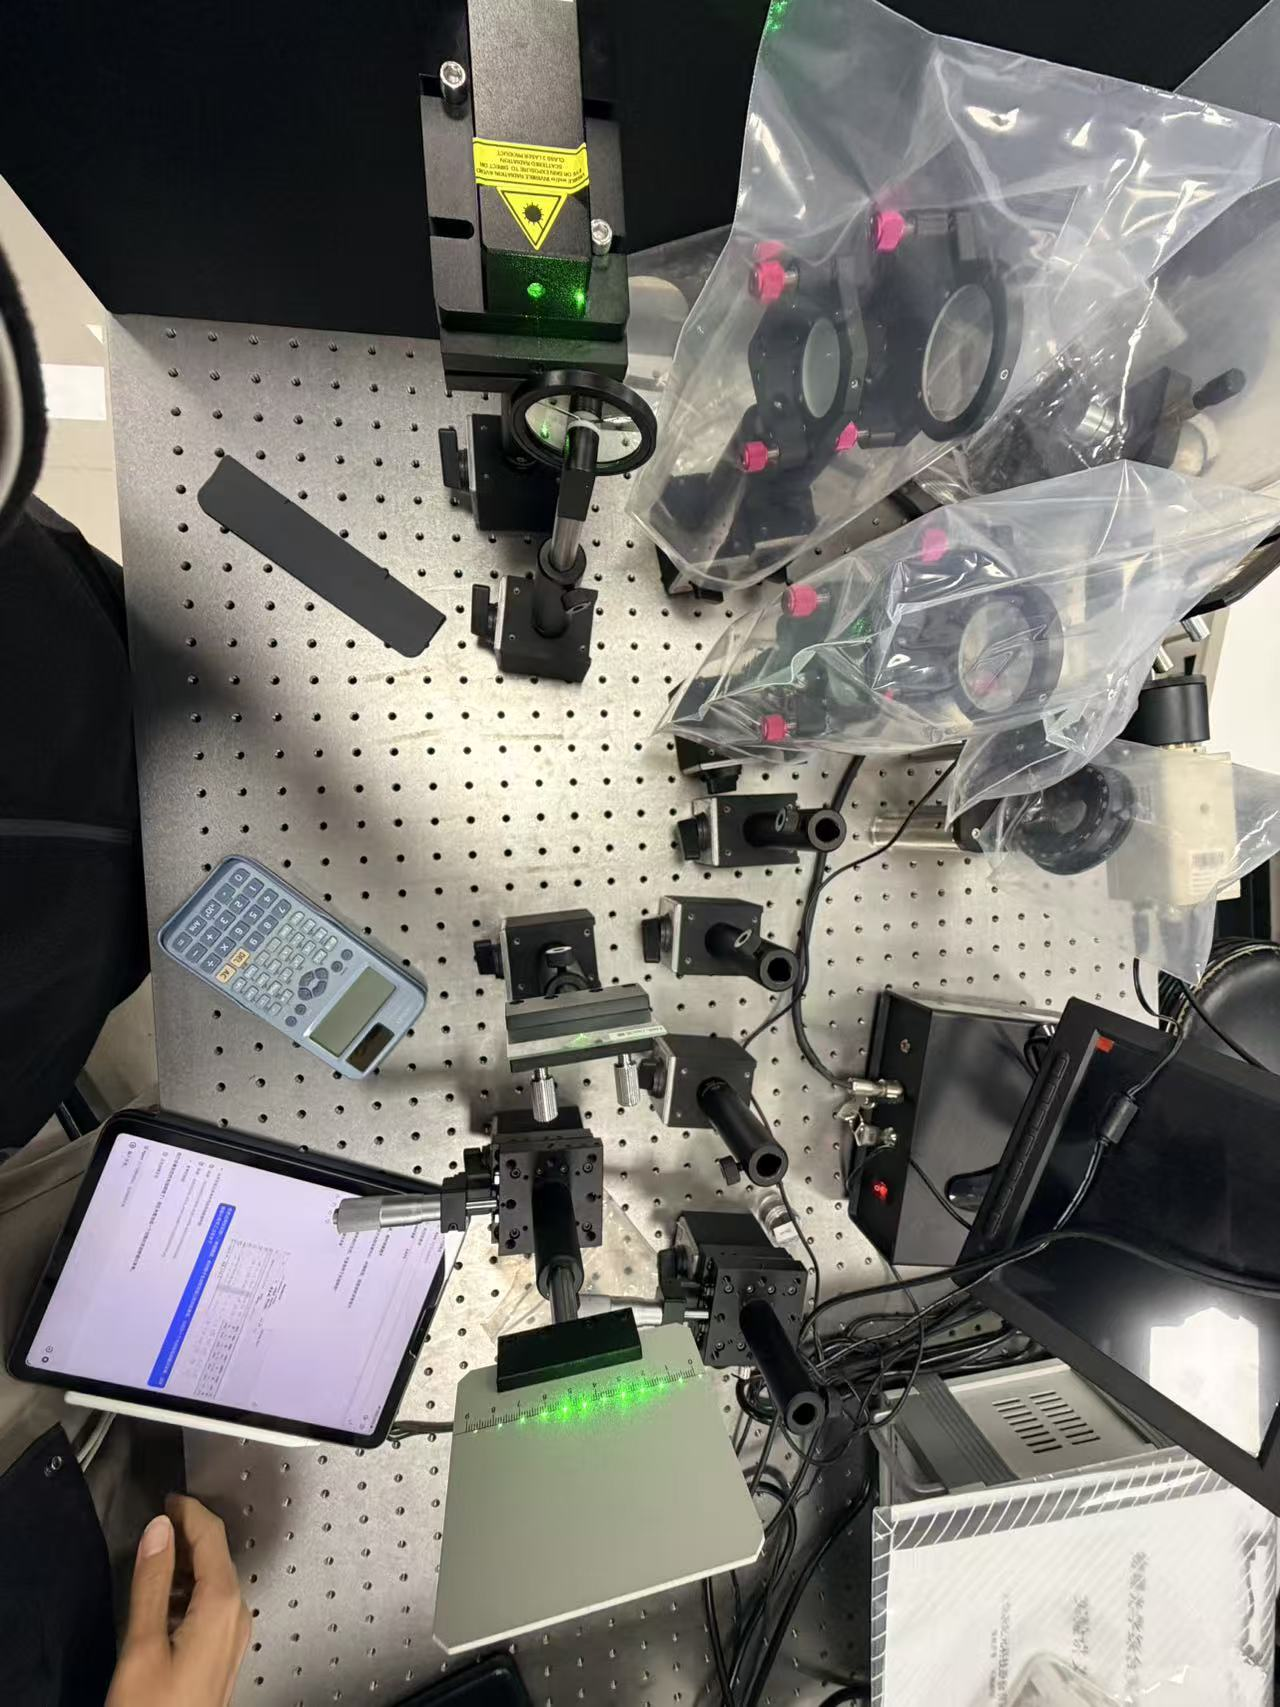
\includegraphics[width=0.75\textwidth]{实验图片/实验二光路搭建.jpg}
\caption{实验二光路实物图}
\label{fig:setup2}
\end{figure}

\subsection{实验三：波长测量与误差分析}

使用已知光栅线数 $N = 100$ 线/mm 的标准光栅（光栅常数 $d = \SI{10}{\micro m}$），在实验一或实验二的基础上，分别测量不同级次衍射光的衍射角，计算各级次的波长测量值及其与标准波长 $\lambda_0 = \SI{532}{nm}$ 的相对误差。

\section{实验数据与处理}

\subsection{实验一：$\pm$5级光栅常数测量}

激光波长 $\lambda = \SI{532}{nm}$，光栅到白屏距离 $L = \SI{15.10}{cm}$，零级位置 $x_0 = \SI{4.52}{cm}$。

\begin{table}[H]
\centering
\caption{实验一：$\pm$5级衍射位置测量数据}
\begin{tabular}{cccccccccccc}
\toprule
级次 $k$ & $-5$ & $-4$ & $-3$ & $-2$ & $-1$ & $0$ & $+1$ & $+2$ & $+3$ & $+4$ & $+5$ \\
\midrule
位置 $x$ (cm) & 0.69 & 1.41 & 2.15 & 2.94 & 3.71 & 4.52 & 5.31 & 6.10 & 6.88 & 7.64 & 8.38 \\
$|x - x_0|$ (cm) & 3.83 & 3.11 & 2.37 & 1.58 & 0.81 & 0 & 0.79 & 1.58 & 2.36 & 3.12 & 3.86 \\
$\tan\theta$ & 0.2536 & 0.2060 & 0.1570 & 0.1046 & 0.0536 & 0 & 0.0523 & 0.1046 & 0.1563 & 0.2066 & 0.2556 \\
$\theta$ ($^\circ$) & 14.23 & 11.64 & 8.92 & 5.97 & 3.07 & 0 & 3.00 & 5.97 & 8.90 & 11.67 & 14.34 \\
$\sin\theta$ & 0.2457 & 0.2016 & 0.1550 & 0.1041 & 0.0536 & 0 & 0.0523 & 0.1041 & 0.1547 & 0.2022 & 0.2476 \\
$d = k\lambda/\sin\theta$ (nm) & 10819 & 10548 & 10293 & 10224 & 9932 & --- & 10182 & 10224 & 10316 & 10517 & 10740 \\
\bottomrule
\end{tabular}
\end{table}

由左右对称级次取平均，计算光栅常数：
\begin{align}
\bar{d} &= \frac{1}{10}\sum_{k=\pm 1}^{\pm 5} d_k = \SI{10381.5}{nm} = \SI{10.38}{\micro m} \\
N &= \frac{1}{d} = \frac{1}{10.38 \times 10^{-3}\,\text{mm}} = 96.3\,\text{线/mm}
\end{align}

\subsection{实验二：$\pm$1级光栅常数测量}

\begin{table}[H]
\centering
\caption{实验二：$\pm$1级衍射测量数据}
\begin{tabular}{cccccccccccc}
\toprule
次数 & $L$ (cm) & $x_{+1}$ (cm) & $x_{-1}$ (cm) & $x_0$ (cm) & $|x_{+1}-x_0|$ (cm) & $|x_{-1}-x_0|$ (cm) & $\bar{x}$ (cm) & $\tan\theta$ & $\theta$ ($^\circ$) & $\sin\theta$ & $d$ (nm) \\
\midrule
1 & 10.93 & 5.13 & 3.98 & 4.55 & 0.58 & 0.57 & 0.575 & 0.0526 & 3.01 & 0.0525 & 10126 \\
2 & 10.54 & 5.24 & 3.50 & 4.48 & 0.76 & 0.98 & 0.87 & 0.0825 & 4.72 & 0.0823 & 10128 \\
\midrule
平均 & 10.74 & --- & --- & --- & --- & --- & 0.723 & 0.0673 & 3.85 & 0.0672 & 7913 \\
\bottomrule
\end{tabular}
\end{table}

实验二结果：光栅常数 $\bar{d} = \SI{7913}{nm} = \SI{7.91}{\micro m}$，光栅线数 $N = 126.4$ 线/mm。

\subsection{实验三：波长测量与误差分析}

使用标准光栅（$N = 100$ 线/mm，$d = \SI{10}{\micro m} = \SI{10000}{nm}$），$L = \SI{15.10}{cm}$。

\begin{table}[H]
\centering
\caption{实验三：不同级次波长测量数据}
\begin{tabular}{cccccccccccc}
\toprule
级次 $k$ & $-5$ & $-4$ & $-3$ & $-2$ & $-1$ & $0$ & $+1$ & $+2$ & $+3$ & $+4$ & $+5$ \\
\midrule
$|x|$ (cm) & 3.83 & 3.11 & 2.37 & 1.58 & 0.81 & 0 & 0.79 & 1.58 & 2.36 & 3.12 & 3.86 \\
$\tan\theta$ & 0.2536 & 0.2060 & 0.1570 & 0.1046 & 0.0536 & 0 & 0.0523 & 0.1046 & 0.1563 & 0.2066 & 0.2556 \\
$\theta$ ($^\circ$) & 14.23 & 11.64 & 8.92 & 5.97 & 3.07 & 0 & 3.00 & 5.97 & 8.90 & 11.67 & 14.34 \\
$\sin\theta$ & 0.2457 & 0.2016 & 0.1550 & 0.1041 & 0.0536 & 0 & 0.0523 & 0.1041 & 0.1547 & 0.2022 & 0.2476 \\
$\lambda$ (nm) & 491.4 & 504.0 & 516.7 & 520.5 & 536.0 & --- & 523.0 & 520.5 & 515.7 & 505.5 & 495.2 \\
$\Delta\lambda$ (nm) & 40.6 & 28.0 & 15.3 & 11.5 & 4.0 & --- & 9.0 & 11.5 & 16.3 & 26.5 & 36.8 \\
$E$ (\%) & 7.63 & 5.26 & 2.88 & 2.16 & 0.75 & --- & 1.69 & 2.16 & 3.06 & 4.98 & 6.92 \\
\bottomrule
\end{tabular}
\end{table}

其中波长计算公式为 $\lambda = d \cdot \sin\theta / k$，绝对误差 $\Delta\lambda = |\lambda - \lambda_0|$，相对误差 $E = (\Delta\lambda / 532) \times 100\%$。

结果汇总：
\begin{itemize}
  \item 最小相对误差：$k = \pm 1$，$E_{\min} = 0.75\%$
  \item 最大相对误差：$k = \pm 5$，$E_{\max} = 7.63\%$
  \item 平均波长 $\bar{\lambda} = \SI{513.8}{nm}$
\end{itemize}

\section{实验结果与分析}

\subsection{光栅常数测量结果}

实验一采用扩束准直光路，测量了 $\pm 1$ 至 $\pm 5$ 共10个级次的衍射位置，通过多组数据平均得到光栅常数 $d = \SI{10.38}{\micro m}$（96.3 线/mm）。实验二采用简化光路，仅测量 $\pm 1$ 级，得到 $d = \SI{7.91}{\micro m}$（126.4 线/mm）。

两次测量结果存在一定差异，主要原因在于：实验二仅使用 $\pm 1$ 级数据进行计算，且两次测量的 $L$ 值不同，距离较短时读数误差对结果影响更大。

\subsection{衍射条纹分布特点}

实验观察到衍射条纹清晰、分布均匀，符合光栅衍射的理论规律。不同级数条纹之间的间距随着衍射级数的增加而逐渐增大，与光栅方程的预测一致。中央零级亮纹强度最大，高级次条纹强度逐渐减弱。实验拍摄的光栅衍射条纹如图 \ref{fig:fringes} 所示。

\begin{figure}[H]
\centering
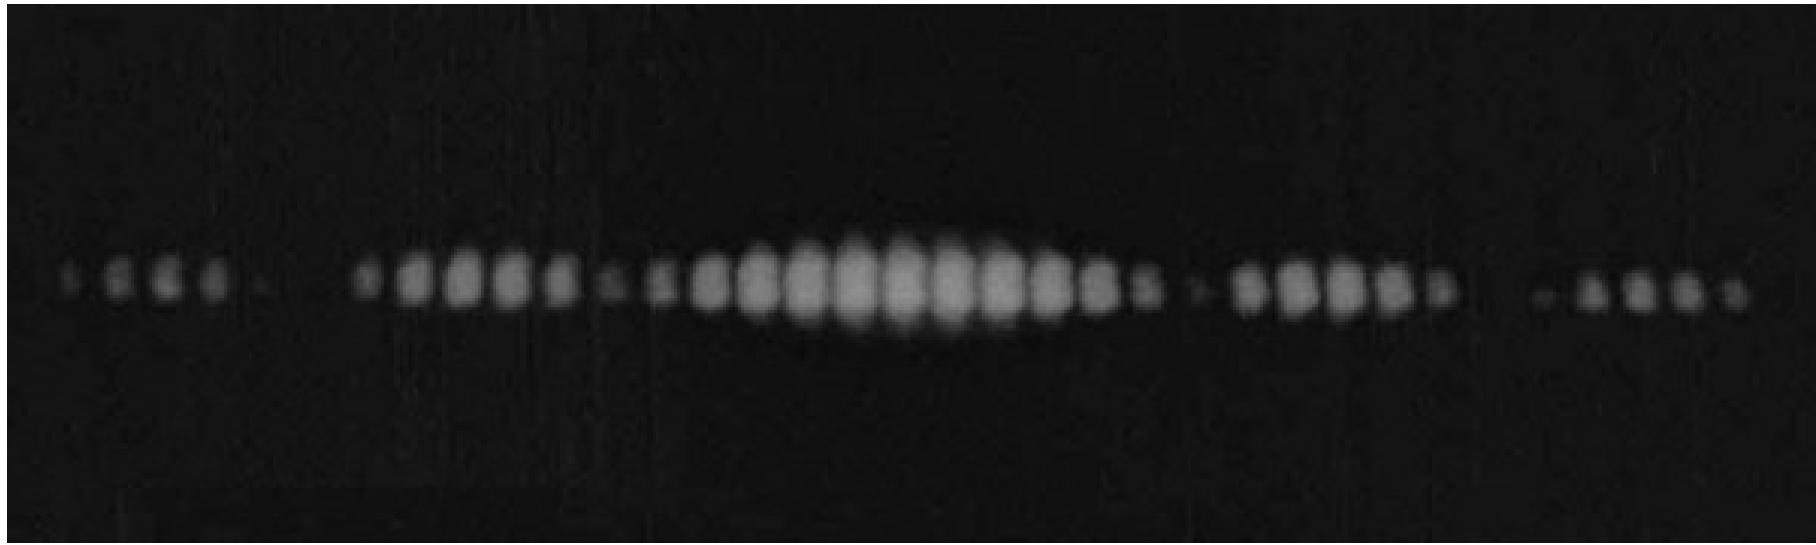
\includegraphics[width=0.85\textwidth]{实验图片/fe45cca0e58e35c0479f5217184fb627ed88844f3af46844b18f2836e1a58d21.jpg}
\caption{光栅衍射条纹}
\label{fig:fringes}
\end{figure}

\subsection{光阑孔径对衍射图案的影响}

当白屏位于聚焦透镜焦平面上时，调节可调光阑的通光孔大小几乎不会改变衍射图案（仅略微变大）。这是因为焦平面上的衍射图样反映了光栅的频谱分布，在通光孔范围内光栅的周期性结构被充分照明，频谱分布基本不变。图 \ref{fig:aperture-large} 和图 \ref{fig:aperture-small} 分别展示了通光孔较大和较小时的衍射图案。

\begin{figure}[H]
\centering
\begin{minipage}[t]{0.48\textwidth}
\centering
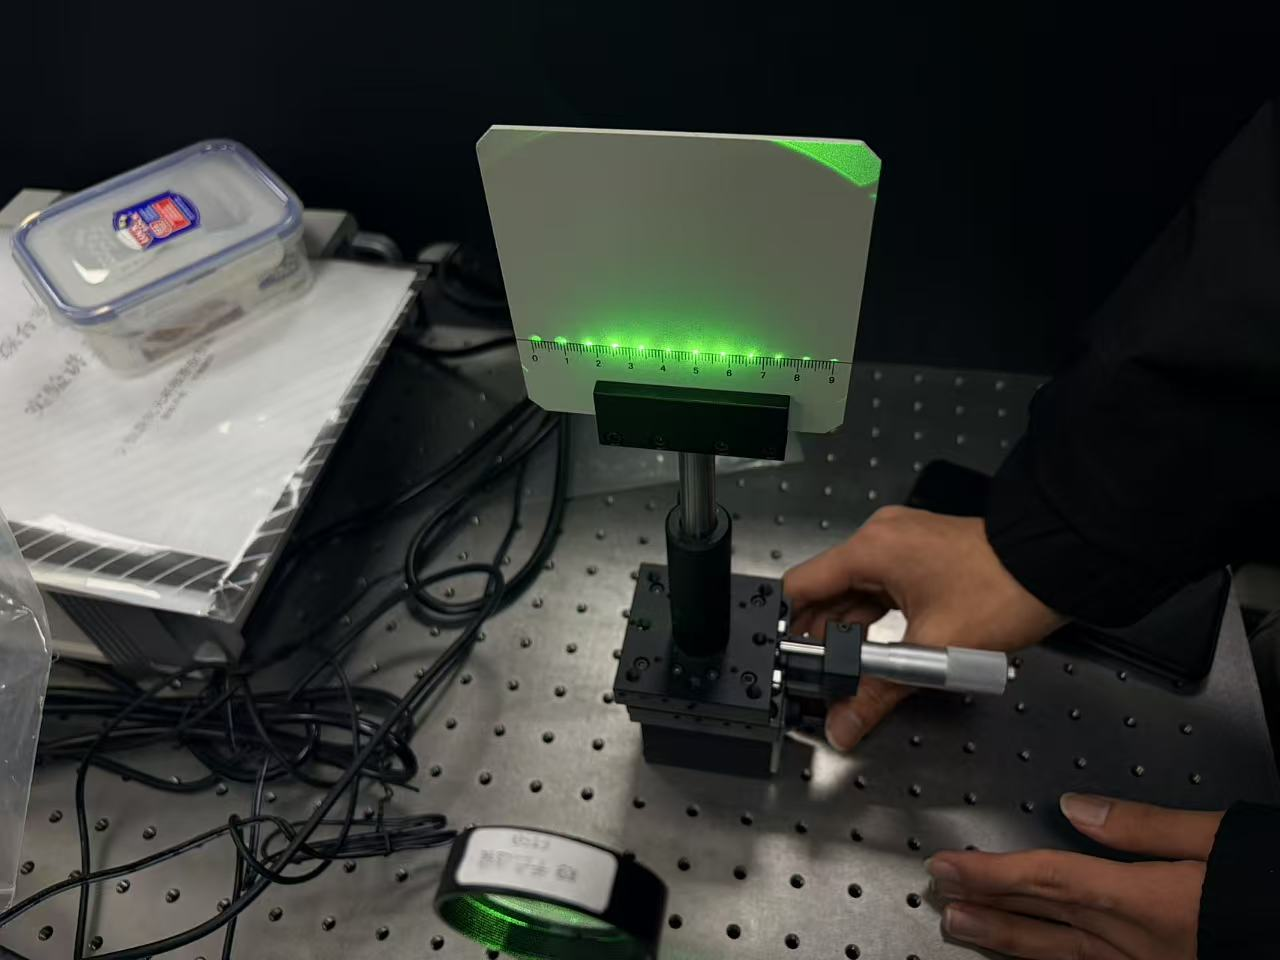
\includegraphics[width=\textwidth]{实验图片/在白屏放在焦平面上时，调节通光孔几乎不会改变衍射图案（略微变大），这是大的场景.jpg}
\caption{通光孔较大时的衍射图案}
\label{fig:aperture-large}
\end{minipage}
\hfill
\begin{minipage}[t]{0.48\textwidth}
\centering
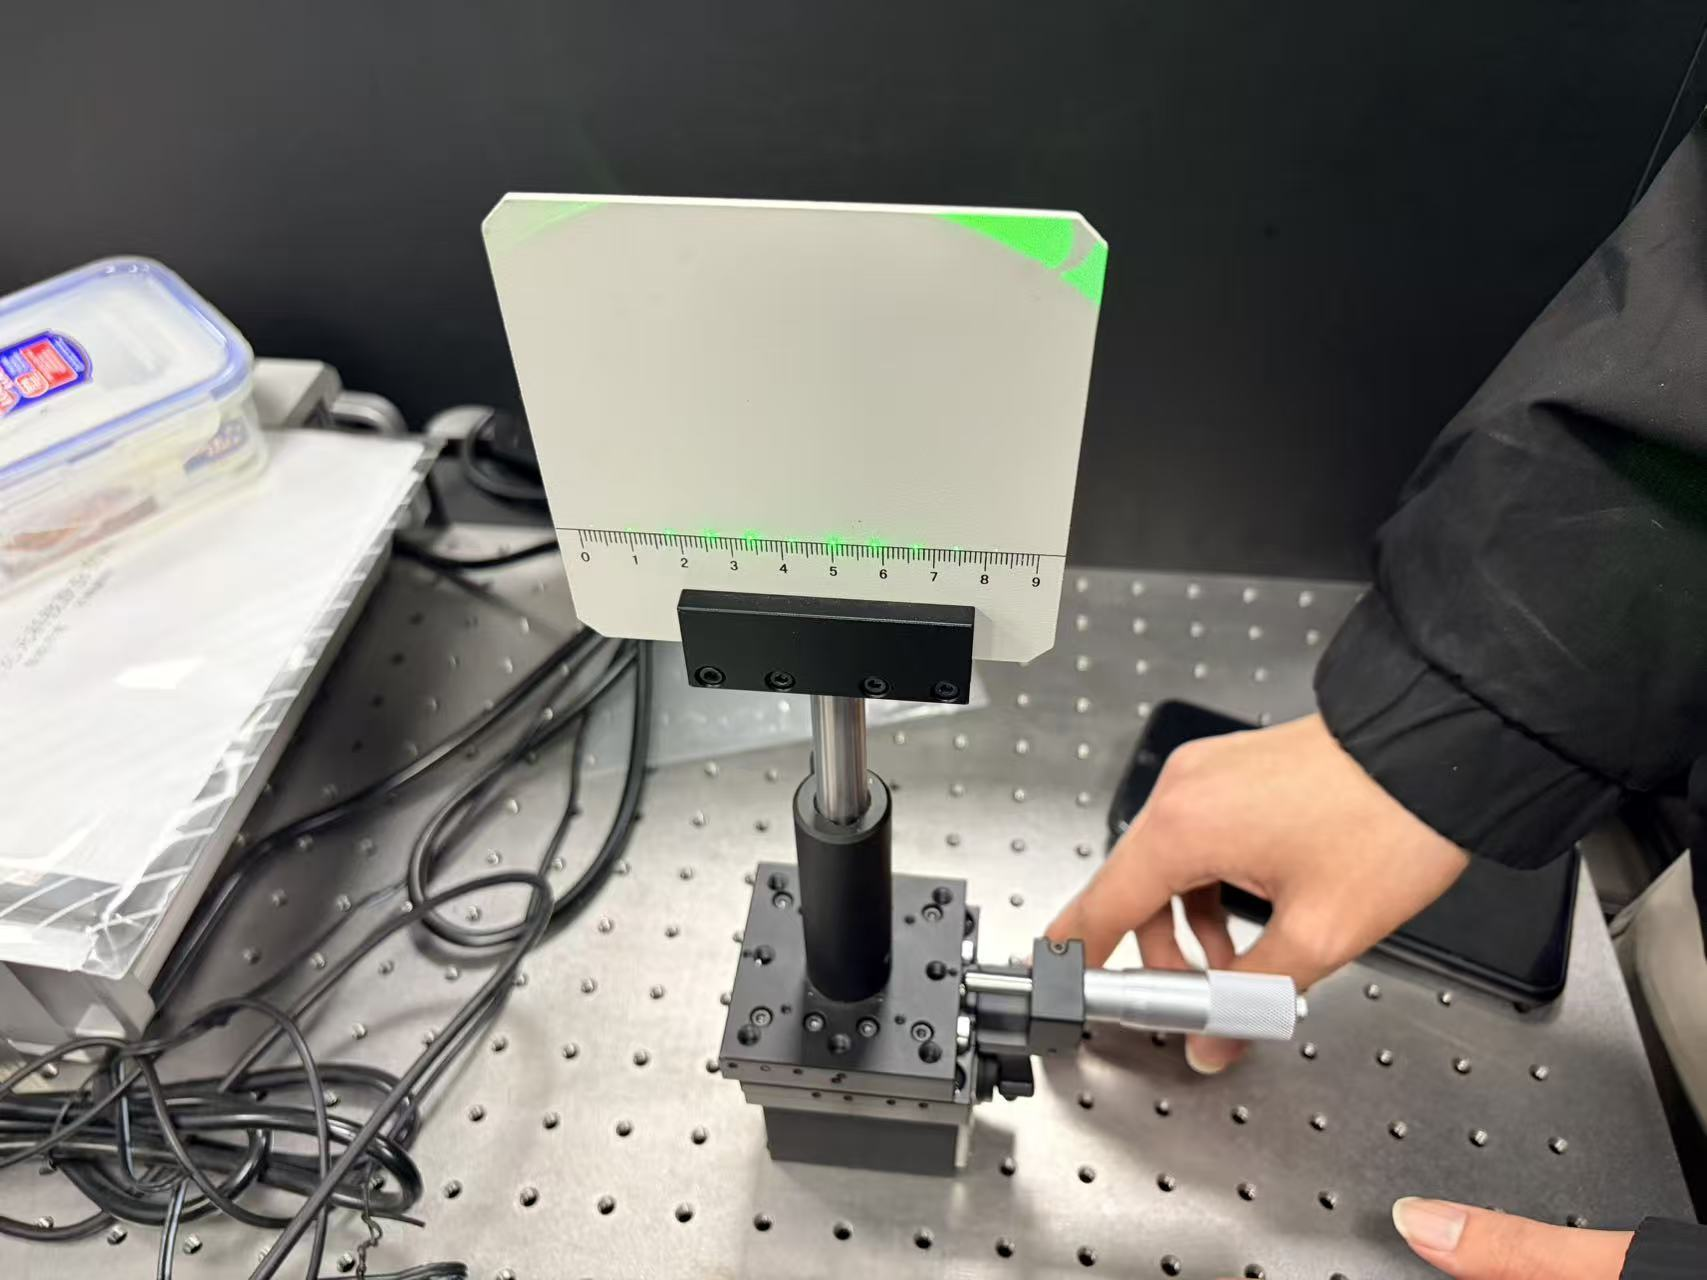
\includegraphics[width=\textwidth]{实验图片/在白屏放在焦平面上时，调节通光孔几乎不会改变衍射图案（略微变大），这是小的场景.jpg}
\caption{通光孔较小时的衍射图案}
\label{fig:aperture-small}
\end{minipage}
\end{figure}

\subsection{离焦对衍射图案的影响}

改变白屏与聚焦透镜的距离（离焦）后，衍射图案不再聚焦，表现为弥散的光斑，如图 \ref{fig:defocus} 所示。只有当白屏位于透镜焦平面时，才能得到清晰的夫琅禾费衍射图样。

\begin{figure}[H]
\centering
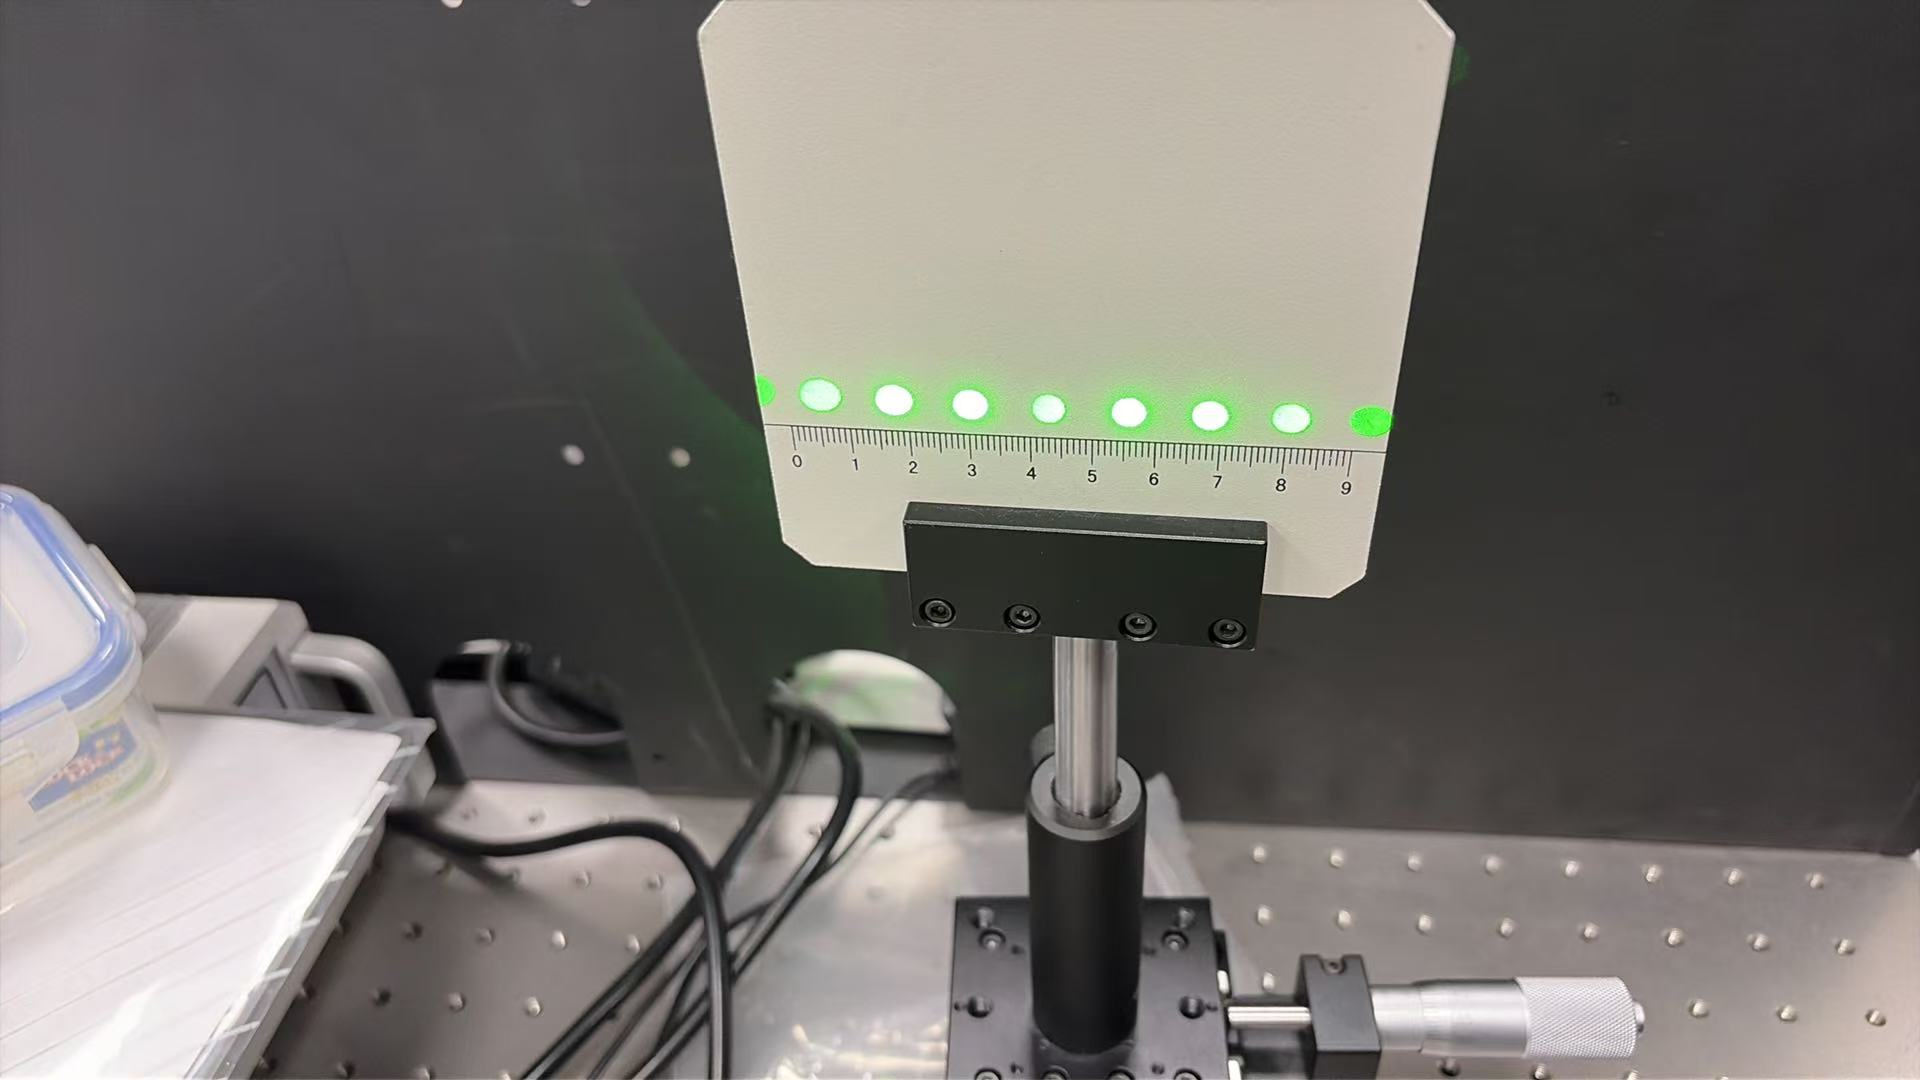
\includegraphics[width=0.75\textwidth]{实验图片/改变白屏与聚焦透镜的距离记录并对比光栅衍射图案的特点，距离拉长之后出现的效果：不再聚焦，变为光斑.jpg}
\caption{离焦后的衍射图案（光斑）}
\label{fig:defocus}
\end{figure}

\section{误差分析}

\subsection{主要误差来源}

\begin{enumerate}
  \item \textbf{距离测量误差}：用卷尺测量光栅到白屏的距离 $L$，估计误差约为 $\pm 0.1\,\text{cm}$，对 $\tan\theta$ 的计算有直接影响。
  
  \item \textbf{位置读数误差}：白屏上的刻度分辨率有限，人工读数存在视差，估计位置读数误差约为 $\pm 0.02\,\text{cm}$。
  
  \item \textbf{光路对准误差}：激光束可能未严格垂直入射光栅平面，导致实际衍射角与理论值存在偏差。根据斜入射光栅方程，入射角 $i$ 的存在会系统性地影响测量结果。
  
  \item \textbf{环境误差}：实验台的振动、空气流动等因素可能导致衍射图样轻微抖动，影响读数精度。
\end{enumerate}

\subsection{误差传递分析}

由光栅方程 $d = k\lambda / \sin\theta$，且 $\tan\theta = x/L$，可得：
\begin{equation}
d = \frac{k\lambda\sqrt{L^2 + x^2}}{x}
\end{equation}

对 $x$ 和 $L$ 求偏导，误差传递公式为：
\begin{equation}
\left(\frac{\Delta d}{d}\right)^2 = \left(\frac{L^2}{x^2(L^2+x^2)}\Delta x\right)^2 + \left(\frac{L}{L^2+x^2}\Delta L\right)^2
\end{equation}

对于 $k = \pm 1$ 级，$x \approx 0.8\,\text{cm}$，$L = 15.10\,\text{cm}$，取 $\Delta x = 0.02\,\text{cm}$，$\Delta L = 0.1\,\text{cm}$，计算得相对误差约为 $2.5\%$，与实验三中 $k = \pm 1$ 级的相对误差 $0.75\%$ 和 $1.69\%$ 基本吻合。

\subsection{改进建议}

\begin{enumerate}
  \item 采用精度更高的位置测量装置（如CCD探测器）替代人工读数；
  \item 增加测量次数，采用最小二乘法拟合处理数据；
  \item 使用准直效果更好的平行光管，确保光束严格垂直入射；
  \item 在防震条件下进行实验，减小环境振动影响。
\end{enumerate}

\section{实验结论}

本实验通过光栅衍射现象测量了透射光栅的光栅常数，主要结论如下：

\begin{enumerate}
  \item 利用 $\pm 5$ 级衍射数据测得光栅常数 $d = \SI{10.38}{\micro m}$（96.3 线/mm），利用 $\pm 1$ 级数据测得 $d = \SI{7.91}{\micro m}$（126.4 线/mm）。多组数据平均可减小随机误差。
  
  \item 实验观察到的衍射条纹清晰、分布均匀，不同级次间距随级数增加而增大，与光栅方程 $d\sin\theta = k\lambda$ 的理论预测一致。
  
  \item 使用标准光栅反测波长时，$k = \pm 1$ 级的测量精度最高（相对误差 $0.75\%$），高级次误差增大，这是因为高级次的 $\sin\theta$ 对角度测量误差更敏感。
  
  \item 验证了夫琅禾费衍射条件（白屏在焦平面）对获得清晰衍射图样的重要性，以及通光孔大小对焦平面上衍射图样的影响规律。
\end{enumerate}

\end{document}
